\chapter{KẾT QUẢ THỰC HIỆN BÀI TOÁN}
\label{chap:chuong3}

Chương này trình bày thiết lập thực nghiệm, kết quả huấn luyện YOLO11s, các thí nghiệm về biển nhỏ, ảnh xấu, so sánh phương pháp truyền thống với học sâu, bộ xác minh, kết quả của hệ thống đầy đủ, tốc độ, chương trình demo và phần thảo luận. Mọi con số được tính bằng script của dự án từ các lần chạy đã ghi trong sổ đăng ký thí nghiệm; các biểu đồ được sinh tự động từ cùng tệp số liệu, không có con số nào chép tay. Trừ khi ghi khác, kết quả được đo trên tập kiểm thử \texttt{processed/v1} (826 ảnh, 2\,017 biển) theo giao thức ở Mục~\ref{sec:protocol}.

\section{Thiết lập thực nghiệm}
\label{sec:setup}

Bảng~\ref{tab:env} tóm tắt môi trường. YOLO11s được huấn luyện một lần (hạt giống 42) trên Google Colab; mọi đánh giá và đo tốc độ chạy trên máy cá nhân của nhóm. Dữ liệu, trọng số và cấu hình của từng lần chạy được ghi lại để tái lập (Phụ lục~\ref{app:code}).

\begin{table}[H]
\centering
\caption{Môi trường thực nghiệm}
\label{tab:env}
\small
\begin{tabularx}{\textwidth}{|>{\raggedright\arraybackslash}p{3.4cm}|>{\raggedright\arraybackslash}X|}
\toprule
\textbf{Hạng mục} & \textbf{Giá trị} \\
\midrule
Huấn luyện YOLO11s & Google Colab, GPU Tesla T4; Python 3.13, PyTorch 2.11 + CUDA 13.0, Ultralytics 8.4.183 \\ \hline
Đánh giá, đo tốc độ & Máy tính xách tay, GPU RTX 4060 Laptop; PyTorch + CUDA 12.6 \\ \hline
Triển khai & Docker Compose (profile CPU và GPU), FastAPI, React 19, Nginx \\ \hline
Thư viện CV / ML & OpenCV 4.14, scikit-image (HOG), scikit-learn 1.9 (SVM), LightGBM 4.7, VietOCR \\ \hline
Dữ liệu & \texttt{processed/v1}, 27 lớp; tập kiểm thử chưa dùng cho bất kỳ lựa chọn nào \\
\bottomrule
\end{tabularx}
\end{table}

\section{Kết quả huấn luyện YOLO11s}
\label{sec:baseline}

\subsection{Quá trình hội tụ}
Hình~\ref{fig:training} cho thấy hàm mất mát khung bao và phân loại trên cả tập huấn luyện lẫn tập xác thực giảm đều đến epoch 80; mất mát xác thực không tăng trở lại, nên không có dấu hiệu quá khớp. Bước giảm đột ngột của mất mát huấn luyện quanh epoch 66 là do tắt tăng cường mosaic ở 15 epoch cuối. mAP@50:95 trên tập xác thực tăng từ 0,645 (epoch 30) lên 0,672 (epoch 50) và 0,685 (epoch 80); 15 epoch cuối chỉ thêm 0,003, tức mô hình gần bão hoà trên dữ liệu hiện có. Thời gian huấn luyện là 2 giờ 52 phút.

\begin{figure}[H]
\centering
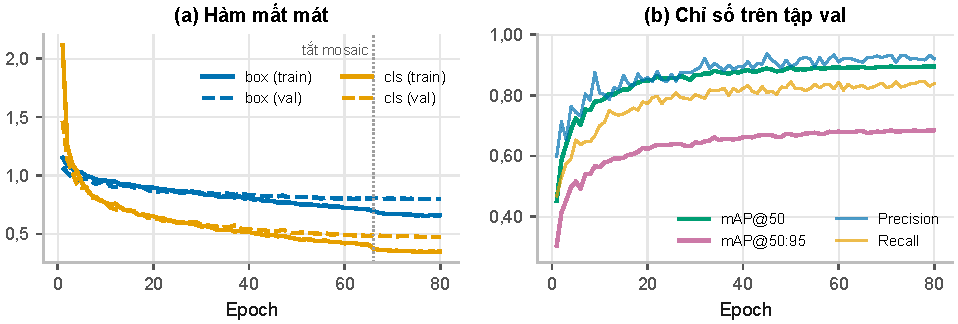
\includegraphics[width=\textwidth]{figures/ch3_huan_luyen.pdf}
\caption{Hàm mất mát (a) và các chỉ số trên tập xác thực (b) của YOLO11s theo epoch}
\label{fig:training}
\end{figure}

\subsection{Kết quả tổng}
Bảng~\ref{tab:baseline} so sánh chỉ số do thư viện báo cáo với chỉ số nhóm tính lại kèm CI 95\% bootstrap 500 lần theo ảnh. Hai cách tính lệch khoảng 0,01 do khác cách đệm ảnh khi suy luận, nên kết quả được báo cáo là mAP@50 $\approx$ 0,89--0,91. Kết quả trên tập xác thực (mAP@50 0,894; mAP@50:95 0,683) tương đương tập kiểm thử, cho thấy việc chọn epoch không quá khớp tập xác thực. Precision 0,920 mà thư viện báo cáo là ở ngưỡng tối ưu theo $F_1$; tại ngưỡng hiển thị $0{,}25$ của hệ thống, precision là 0,860.

\begin{table}[H]
\centering
\caption{Kết quả YOLO11s (suy luận 960 px) trên tập kiểm thử}
\label{tab:baseline}
\small
\begin{tabularx}{\textwidth}{|>{\raggedright\arraybackslash}X|>{\centering\arraybackslash}p{3cm}|>{\centering\arraybackslash}p{3cm}|>{\centering\arraybackslash}p{3.4cm}|}
\toprule
\textbf{Chỉ số} & \textbf{Ultralytics} & \textbf{Tính lại} & \textbf{CI 95\% (bootstrap)} \\
\midrule
mAP@50 & 0,905 & 0,892 & [0,868; 0,917] \\ \hline
mAP@50:95 & 0,684 & 0,676 & [0,657; 0,702] \\ \hline
Precision tại điểm $0{,}25$ & -- & 0,860 & [0,842; 0,878] \\ \hline
Recall tại điểm $0{,}25$ & -- & 0,893 & [0,875; 0,913] \\
\bottomrule
\end{tabularx}
\end{table}

\subsection{Theo kích thước biển}
Bảng~\ref{tab:size_s1} phân tích từng biển thật của tập xác thực và kiểm thử tại ngưỡng $0{,}25$. Với biển từ 16~px trở lên, khoảng 95\% được nhận đúng; lỗi tập trung ở biển dưới 16~px: chỉ 61,7\% được nhận đúng và 32,8\% bị bỏ sót. Nhầm lớp chiếm tỉ lệ nhỏ ở mọi nhóm. Điều này xác định điểm yếu chính của mô hình là \textit{tìm} biển nhỏ, không phải \textit{phân loại} sai.

\begin{table}[H]
\centering
\caption{Kết quả của YOLO11s theo kích thước biển (val + test, ngưỡng $0{,}25$)}
\label{tab:size_s1}
\small
\begin{tabularx}{\textwidth}{|>{\raggedright\arraybackslash}X|>{\centering\arraybackslash}p{2.2cm}|>{\centering\arraybackslash}p{2.2cm}|>{\centering\arraybackslash}p{2.2cm}|>{\centering\arraybackslash}p{2.2cm}|}
\toprule
\textbf{Cạnh biển} & \textbf{Số biển} & \textbf{Đúng lớp} & \textbf{Sai lớp} & \textbf{Bỏ sót} \\
\midrule
$<16$ px & 702 & 0,617 & 0,056 & \textbf{0,328} \\ \hline
$16$--$32$ px & 1\,427 & 0,922 & 0,036 & 0,043 \\ \hline
$32$--$64$ px & 1\,261 & 0,964 & 0,013 & 0,023 \\ \hline
$\ge64$ px & 636 & 0,975 & 0,003 & 0,022 \\
\bottomrule
\end{tabularx}
\end{table}

\subsection{Theo lớp}
Hình~\ref{fig:per_class} cho recall của 27 lớp kèm CI Wilson. 24/27 lớp có recall từ 0,81 trở lên. Ba lớp yếu nhất đều có nguyên nhân xác định:
\begin{itemize}
 \item \textit{Vạch sang đường cho người đi bộ} (recall 0,57, $n=30$) và \textit{Giới hạn chiều cao} (0,68, $n=65$): 57\% và 34\% số biển nhỏ hơn 16~px; với biển từ 16~px trở lên, recall đạt 1,00 và 0,84.
 \item \textit{Biển chỉ dẫn hướng đi} (recall 0,70, precision 0,60): nhãn gốc gộp cả bảng chỉ dẫn chữ nhật lẫn biển tròn xanh, nên định nghĩa lớp không nhất quán; vấn đề nằm ở dữ liệu, không thể sửa vì dữ liệu đã đóng băng.
\end{itemize}
Số lượng dữ liệu tương quan yếu với chất lượng lớp (hệ số Spearman 0,16--0,32 giữa số cụm cảnh và recall/AP). Các lớp hiếm vẫn đạt recall 0,81--0,97 nhưng CI rộng vì chỉ có 23--31 biển để đánh giá. Các cặp nhầm lẫn lớn nhất chỉ chiếm tối đa 6\% số biển của lớp: Biển gộp làn đường $\leftrightarrow$ Biển chỉ dẫn hướng đi, Cấm dừng và đỗ xe $\leftrightarrow$ Cấm đỗ xe, Giới hạn tốc độ $\rightarrow$ Biển cấm phương tiện.

\begin{figure}[H]
\centering
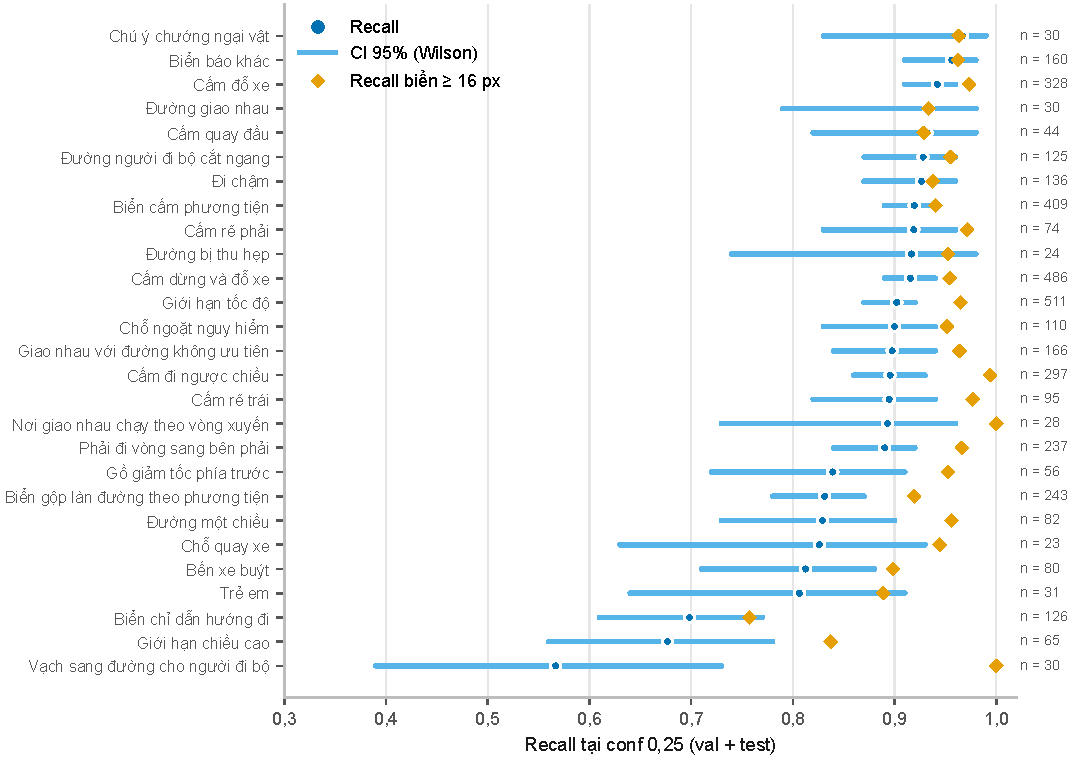
\includegraphics[width=.94\textwidth]{figures/ch3_theo_lop.pdf}
\caption{Recall theo lớp của YOLO11s (val + test, ngưỡng $0{,}25$) kèm CI 95\% Wilson}
\label{fig:per_class}
\end{figure}

\subsection{Theo mức tương đồng với tập huấn luyện}
\label{sec:similarity}
Dù dữ liệu được chia theo cụm và không ảnh kiểm thử nào gần trùng ảnh huấn luyện (khoảng cách pHash $\le6$), khoảng một phần ba ảnh kiểm thử vẫn khá giống ảnh huấn luyện (cùng tuyến đường, cùng camera). Hình~\ref{fig:similarity} chia ảnh kiểm thử theo khoảng cách pHash tới ảnh huấn luyện gần nhất. Kết quả giảm rõ khi cảnh càng khác: recall từ 0,978 xuống 0,805 và precision từ 0,942 xuống 0,749. Ngay cả khi chỉ xét biển từ 16~px trở lên, recall vẫn giảm từ 0,978 xuống 0,893, và precision giảm mạnh nhất: cảnh lạ sinh nhiều phát hiện sai trên nền. Kết quả trên nhóm ``khác train'' là ước lượng gần hơn cho ảnh của tuyến đường mới.

\begin{figure}[H]
\centering
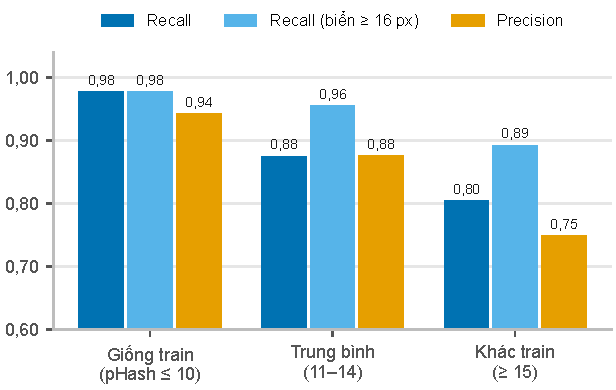
\includegraphics[width=.72\textwidth]{figures/ch3_tuong_dong.pdf}
\caption{Kết quả của YOLO11s theo mức tương đồng của ảnh kiểm thử với tập huấn luyện}
\label{fig:similarity}
\fignote{Số ảnh / số biển: 243 / 667 (giống), 271 / 746 (trung bình), 265 / 604 (khác).}
\end{figure}

\section{Biển nhỏ: độ phân giải suy luận và cắt ô (T3)}
\label{sec:t3}

Vì không thể bổ sung dữ liệu, nhóm thử hai cách tăng recall biển nhỏ mà không cần huấn luyện lại: tăng kích thước ảnh khi suy luận lên 1280 px và cắt ảnh thành các ô 640 px chồng lấn theo kiểu SAHI~\cite{akyon2022sahi}. Kết quả ở Bảng~\ref{tab:t3} và Hình~\ref{fig:t3}.

\begin{table}[H]
\centering
\caption{Ảnh hưởng của cách suy luận đến biển nhỏ (cùng trọng số huấn luyện ở 960 px)}
\label{tab:t3}
\small
\begin{tabularx}{\textwidth}{|>{\raggedright\arraybackslash}X|>{\centering\arraybackslash}p{1.9cm}|>{\centering\arraybackslash}p{1.6cm}|>{\centering\arraybackslash}p{1.6cm}|>{\centering\arraybackslash}p{2.3cm}|>{\centering\arraybackslash}p{1.9cm}|}
\toprule
\textbf{Cách suy luận} & \textbf{Precision} & \textbf{Recall} & \textbf{$F_1$} & \textbf{Recall $<16$ px} & \textbf{ms / ảnh} \\
\midrule
960 px (như khi huấn luyện) & 0,861 & 0,893 & 0,877 & 0,634 & 18,6 \\ \hline
\textbf{1280 px (mặc định)} & \textbf{0,861} & 0,917 & \textbf{0,888} & 0,737 & 21,4 \\ \hline
960 px + cắt ô 640 & 0,749 & \textbf{0,932} & 0,831 & \textbf{0,784} & 46,5 \\
\bottomrule
\end{tabularx}
\tablenote{GPU RTX 4060 Laptop; thời gian chỉ gồm khâu phát hiện.}
\end{table}

\begin{figure}[H]
\centering
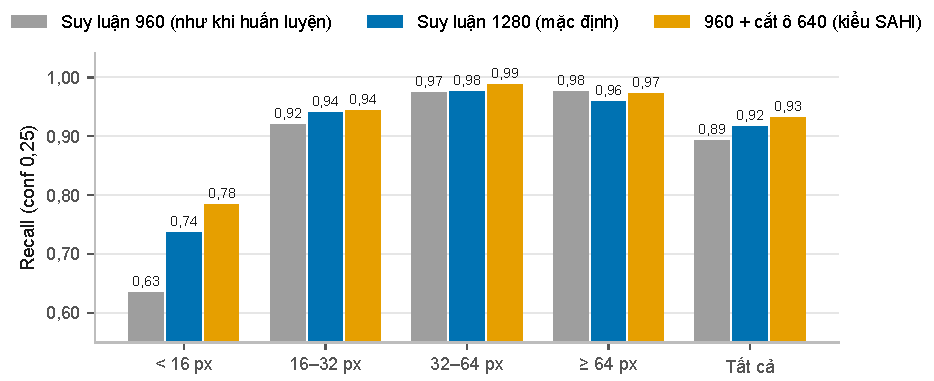
\includegraphics[width=\textwidth]{figures/ch3_t3_kich_thuoc.pdf}
\caption{Recall theo kích thước biển với ba cách suy luận}
\label{fig:t3}
\end{figure}

Suy luận ở 1280 px tăng recall biển dưới 16~px thêm 10,3 điểm (0,634 $\rightarrow$ 0,737) mà precision giữ nguyên và chỉ chậm thêm khoảng 15\%; recall biển từ 64~px giảm nhẹ (0,976 $\rightarrow$ 0,958) vì một số biển lớn bị phóng quá kích thước mô hình đã học. Cắt ô cho recall cao nhất nhưng precision giảm 0,11 do ô cắt làm mất ngữ cảnh và tạo nhiều phát hiện sai ở mép ô, đồng thời chậm 2,5 lần. Nhóm chọn 1280 px làm mặc định và giữ cắt ô làm tuỳ chọn cho ảnh tĩnh độ phân giải cao.

\section{Tăng cường ảnh khi điều kiện xấu (T4, E4)}
\label{sec:t4}

826 ảnh kiểm thử được làm xấu nhân tạo rồi đưa qua YOLO11s (960 px) theo ba chế độ: không xử lý, tăng cường thích nghi của hệ thống (Mục~\ref{sec:enhance}) và luôn áp gamma + CLAHE cho mọi ảnh (đối chứng). Bảng~\ref{tab:t4} cho kết quả kèm CI bootstrap ghép cặp 1\,000 lần theo ảnh.

\begin{table}[H]
\centering
\caption{Recall của YOLO11s khi ảnh bị làm xấu, với ba chế độ tăng cường}
\label{tab:t4}
\small
\begin{tabularx}{\textwidth}{|>{\raggedright\arraybackslash}p{2.6cm}|>{\centering\arraybackslash}p{1.8cm}|>{\centering\arraybackslash}X|>{\centering\arraybackslash}X|}
\toprule
\textbf{Điều kiện} & \textbf{Không xử lý} & \textbf{Thích nghi: \% ảnh xử lý; R; $\Delta$R (CI 95\%)} & \textbf{Luôn gamma + CLAHE: R; $\Delta$R (CI 95\%)} \\
\midrule
Ảnh gốc & 0,893 & 2,8\%; 0,892; $-0{,}001$ ($-0{,}003$; $0{,}000$) & 0,890; $-0{,}003$ ($-0{,}010$; $+0{,}004$) \\ \hline
Tối ($\gamma$ 2,5) & 0,810 & 68,2\%; 0,853; $\mathbf{+0{,}044}$ ($+0{,}032$; $+0{,}056$) & 0,873; $+0{,}063$ ($+0{,}049$; $+0{,}077$) \\ \hline
Rất tối ($\gamma$ 3,5) & 0,686 & 80,5\%; \textbf{0,822}; $\mathbf{+0{,}136}$ ($+0{,}116$; $+0{,}155$) & 0,854; $+0{,}168$ ($+0{,}147$; $+0{,}188$) \\ \hline
Nhiễu ($\sigma$ 15) & 0,799 & 2,8\%; 0,799; $0{,}000$ ($-0{,}001$; $+0{,}001$) & 0,706; $\mathbf{-0{,}093}$ ($-0{,}109$; $-0{,}077$) \\ \hline
Mờ chuyển động & 0,748 & 2,8\%; 0,748; $0{,}000$ ($-0{,}001$; $+0{,}002$) & 0,734; $-0{,}014$ ($-0{,}024$; $-0{,}004$) \\
\bottomrule
\end{tabularx}
\end{table}

\begin{figure}[H]
\centering
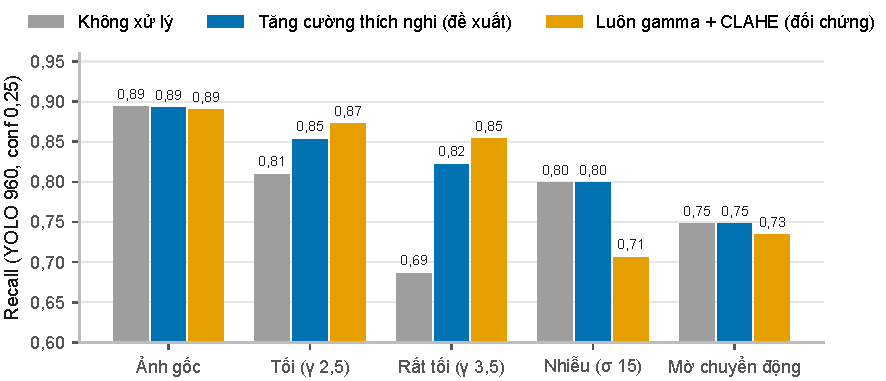
\includegraphics[width=\textwidth]{figures/ch3_t4_tang_cuong.pdf}
\caption{Recall của YOLO11s trên ảnh bị làm xấu với ba chế độ tăng cường}
\label{fig:t4}
\end{figure}

Ba nhận xét rút ra từ Bảng~\ref{tab:t4} và Hình~\ref{fig:t4}:
\begin{enumerate}
 \item \textbf{Tăng cường truyền thống có tác dụng rõ với ảnh tối.} Chế độ thích nghi khôi phục 53\% ($\gamma$ 2,5) và 66\% ($\gamma$ 3,5) phần recall bị mất, có ý nghĩa thống kê, và đạt yêu cầu recall $\ge0{,}80$ trên ảnh rất tối. Precision giảm nhẹ (khoảng 0,02) vì ảnh sáng hơn làm lộ thêm vật thể giống biển.
 \item \textbf{Bước đánh giá chất lượng là cần thiết.} Áp CLAHE cho mọi ảnh làm hại ảnh nhiễu (recall giảm 0,093) và ảnh mờ, vì CLAHE khuếch đại cả nhiễu. Chế độ thích nghi không kích hoạt ở các trường hợp này nên không gây hại, và gần như không chạm vào ảnh tốt (2,8\% ảnh gốc).
 \item \textbf{Hạn chế.} Ngưỡng tối $\mu_V<0{,}30$ bỏ sót 20--32\% ảnh đã làm tối, nên chế độ thích nghi kém hơn ``luôn áp'' trên ảnh tối. Phương sai Laplacian không phân biệt được nhiễu Gauss với chi tiết thật như tán lá, nên lọc song phương chưa được kích hoạt trong thí nghiệm này; chưa có bằng chứng về tác dụng khử nhiễu.
\end{enumerate}

Khi đưa vào hệ thống đầy đủ (E4, suy luận 1280 px, ảnh tối $\gamma$ 2,5), hệ thống đạt precision 0,884, recall 0,866 và $F_1$ 0,875. Hình~\ref{fig:dark} minh hoạ trên một ảnh làm tối $\gamma$ 3,5: sau khi bộ đánh giá chất lượng chọn gamma và CLAHE ($\mu_V=0{,}14$), YOLO11s tìm thêm các biển ở mép phải ảnh mà ảnh tối bỏ sót.

\begin{figure}[H]
\centering
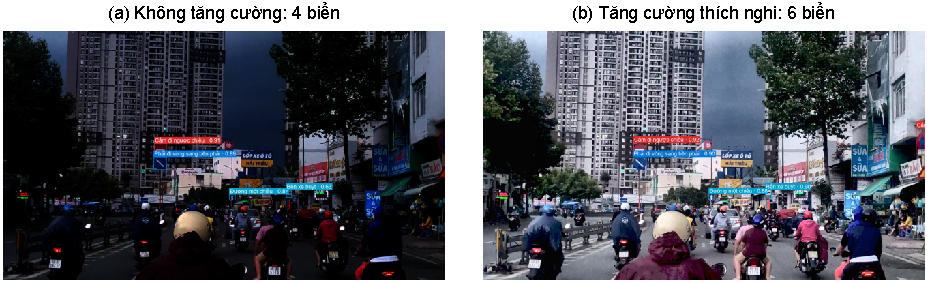
\includegraphics[width=\textwidth]{figures/ch3_anh_toi.pdf}
\caption{Ảnh kiểm thử làm tối ($\gamma$ 3,5) trước và sau tăng cường thích nghi}
\label{fig:dark}
\end{figure}

\section{So sánh đặc trưng thủ công và học sâu (E8)}
\label{sec:e8}

\subsection{Thiết kế so sánh}
Theo cách tách đánh giá của GTSRB và GTSDB~\cite{stallkamp2012gtsrb,houben2013gtsdb}, thí nghiệm E8 so sánh riêng khâu \textit{phân loại} trên cùng 2\,017 biển kiểm thử. Các phương pháp truyền thống (HOG + SVM, HOG + màu + SVM, SIFT-BoVW + SVM) được huấn luyện trên 9\,449 vùng biển của tập huấn luyện, chọn $C$ trên 2\,009 vùng của tập xác thực và được \textit{cho sẵn vị trí biển} (vùng cắt từ nhãn thật, nới 10\%). YOLO11s phải tự tìm biển: lớp của nó là lớp của dự đoán có điểm cao nhất với IoU $\ge0{,}5$; nếu không có thì tính là sai. Vì phương pháp truyền thống có lợi thế được cho vị trí, phép so sánh công bằng là trên 1\,956 biển mà YOLO tìm thấy (cùng tập mẫu cho mọi phương pháp).

\subsection{Kết quả}

\begin{table}[H]
\centering
\caption{Phân loại biển: đặc trưng thủ công + SVM so với YOLO11s (tập kiểm thử)}
\label{tab:e8}
\small
\begin{tabularx}{\textwidth}{|>{\raggedright\arraybackslash}X|>{\centering\arraybackslash}p{3.0cm}|>{\centering\arraybackslash}p{1.6cm}|>{\centering\arraybackslash}p{2.5cm}|>{\centering\arraybackslash}p{1.6cm}|}
\toprule
\textbf{Phương pháp} & \textbf{Accuracy (CI 95\%)} & \textbf{Macro-$F_1$} & \textbf{Acc.\ trên biển YOLO tìm thấy} & \textbf{ms / vùng} \\
\midrule
SIFT-BoVW + SVM & 0,711 (0,691--0,730) & 0,662 & 0,724 & 2,7 \\ \hline
HOG + SVM & 0,888 (0,874--0,901) & 0,852 & 0,901 & 1,6 \\ \hline
HOG + màu + SVM & 0,910 (0,897--0,922) & 0,872 & 0,920 & 2,0 \\ \hline
\textbf{YOLO11s} & \textbf{0,924} (0,912--0,935) & \textbf{0,917} & \textbf{0,953} & 22$^{*}$ \\
\bottomrule
\end{tabularx}
\tablenote{$^{*}$ms trên mỗi ảnh, gồm cả tìm biển (GPU); các phương pháp truyền thống chạy trên CPU.}
\end{table}

\begin{figure}[H]
\centering
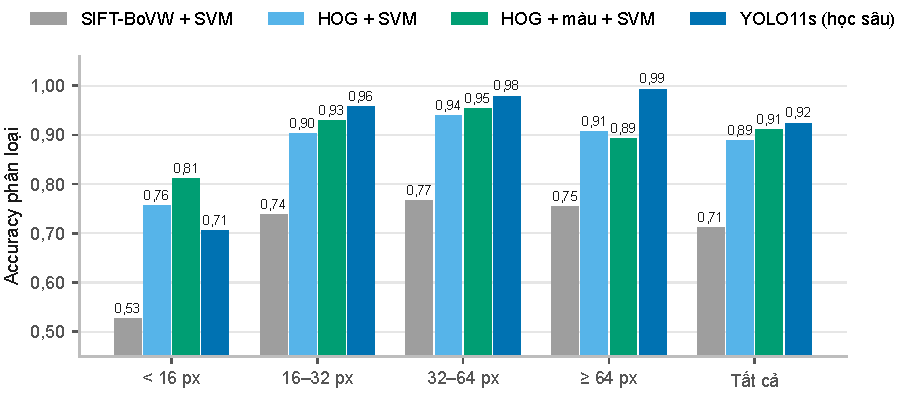
\includegraphics[width=\textwidth]{figures/ch3_e8_phan_loai.pdf}
\caption{Accuracy phân loại theo kích thước biển của bốn phương pháp}
\label{fig:e8}
\fignote{Phương pháp truyền thống được cho sẵn vị trí biển; YOLO11s bị tính sai cả khi bỏ sót biển.}
\end{figure}

\begin{figure}[H]
\centering
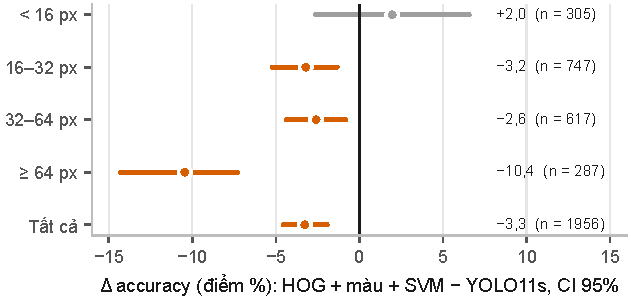
\includegraphics[width=.8\textwidth]{figures/ch3_e8_ghep_cap.pdf}
\caption{Chênh lệch accuracy ghép cặp giữa HOG + màu + SVM và YOLO11s trên các biển YOLO tìm thấy (bootstrap 2\,000 lần)}
\label{fig:e8_paired}
\fignote{Màu đỏ: CI 95\% không chứa 0 (khác biệt có ý nghĩa); màu xám: không khác biệt.}
\end{figure}

Từ Bảng~\ref{tab:e8}, Hình~\ref{fig:e8} và Hình~\ref{fig:e8_paired}:
\begin{enumerate}
 \item \textbf{Đặc trưng thủ công cạnh tranh được ở khâu phân loại.} HOG + màu + SVM chỉ kém YOLO11s 1,4 điểm accuracy tổng. Thêm histogram màu HSV vào HOG tăng 2,2 điểm: màu là thông tin quy chuẩn mà HOG trên ảnh xám bỏ qua. Kết quả 91,0\% cùng mức với HOG-SVM trên GTSRB (89,65--91,25\%~\cite{vieira2025hogsvm}), dù không so sánh trực tiếp được vì khác dữ liệu.
 \item \textbf{Với biển nhỏ, điểm yếu của YOLO là tìm biển, không phải phân loại.} YOLO bỏ sót 15,5\% số biển dưới 16~px. Trên các biển nhỏ mà YOLO tìm thấy, hai phương pháp ngang nhau: chênh lệch $+2{,}0$ điểm, CI 95\% từ $-2{,}6$ đến $+6{,}6$. Khi được cho vị trí, HOG + màu đúng 81,2\% số biển nhỏ, so với 70,6\% của YOLO (tính cả biển bỏ sót).
 \item \textbf{Biển lớn là nơi đặc trưng thủ công thua rõ nhất} ($-10{,}4$ điểm, CI từ $-14{,}3$ đến $-7{,}3$). Thu vùng về $32\times32$ làm mất chi tiết của biển chỉ dẫn và biển có chữ, trong khi CNN học đặc trưng ở nhiều tỉ lệ.
 \item \textbf{SIFT không phù hợp với biển báo.} SIFT-BoVW kém HOG 17,7 điểm. Số điểm SIFT trung vị chỉ là 1 với biển dưới 16~px (93\% số biển có dưới 5 điểm), 8 với biển 16--32~px và 74 với biển từ 64~px. Biển báo là vùng phẳng với ký hiệu đơn giản, ít điểm góc và kết cấu, nên điểm khoá chủ yếu nằm trên viền tròn chung của nhiều lớp.
 \item \textbf{Đặc trưng thủ công rẻ} (1,6--2,7 ms mỗi vùng trên CPU) nhưng cần một bước định vị riêng --- chính là phần YOLO làm tốt.
\end{enumerate}

\subsection{So sánh hai hệ thống trên cùng ảnh}
Khác với E8, Hình~\ref{fig:qualitative} so sánh \textit{toàn bộ} hai hệ thống, gồm cả bước định vị: YOLO11s và pipeline đối chứng (màu + hình dạng + HOG + SVM). Trên ảnh có 16 biển được gán nhãn (hàng đầu), YOLO11s trả 22 phát hiện, còn pipeline truyền thống chỉ trả 8; số phát hiện của YOLO lớn hơn số nhãn vì có cả biển ở xa không được gán nhãn và một số phát hiện trùng. Pipeline truyền thống gộp các biển cùng màu đứng sát nhau thành một vùng, bỏ sót biển chỉ dẫn nhiều màu và biển rất nhỏ, và báo nhầm trên vùng đỏ như áo người đi xe máy (hàng giữa). Khi YOLO11s cung cấp vị trí, HOG + màu + SVM đồng ý với YOLO ở 14/22 biển của ảnh hàng đầu. Như vậy, trong hệ thống truyền thống, bước định vị bằng màu--hình dạng mới là nút thắt, không phải bước phân loại.

\begin{figure}[H]
\centering
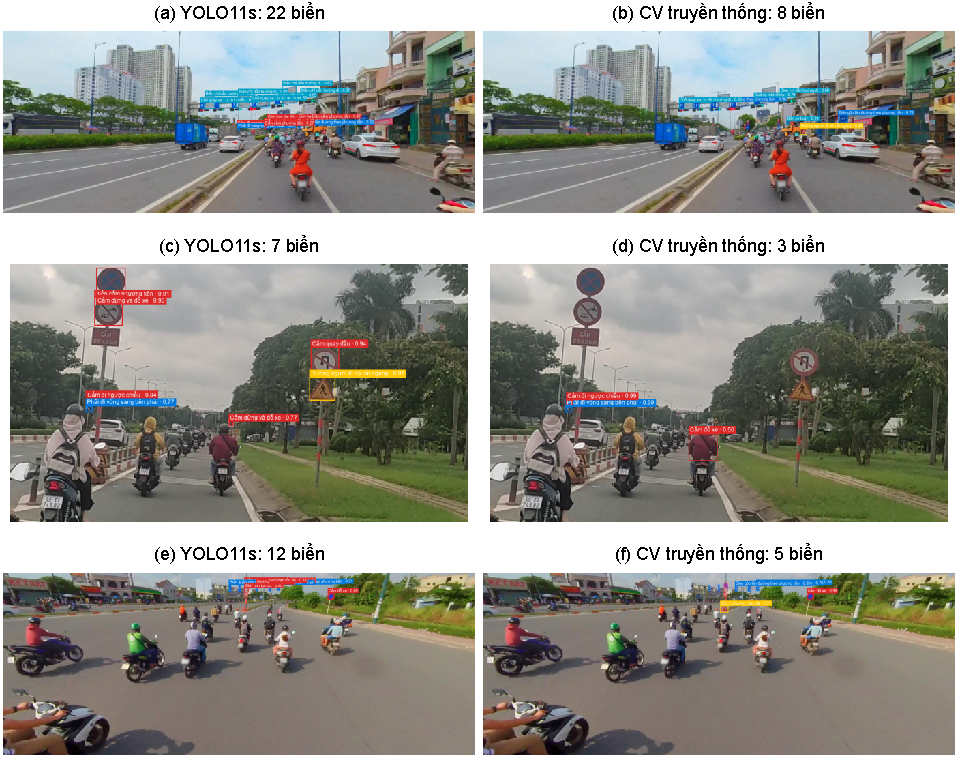
\includegraphics[width=\textwidth]{figures/ch3_dinh_tinh.pdf}
\caption{Kết quả của YOLO11s (trái) và pipeline CV truyền thống (phải) trên ba ảnh của tập kiểm thử}
\label{fig:qualitative}
\fignote{Cùng ảnh đầu vào, cùng khâu tăng cường thích nghi; số biển là số phát hiện mà mỗi hệ thống trả về.}
\end{figure}

\section{Bộ xác minh bằng đặc trưng thủ công (T0, T1)}
\label{sec:t1}

Thí nghiệm T0 cho thấy dư địa lý thuyết của bộ xác minh là lớn: 68--71\% phát hiện sai của YOLO11s là vùng nền (phần còn lại là sai lớp 21--25\% và định vị kém 4--8\%, tuỳ tập và ngưỡng) --- đúng loại lỗi mà màu và hình dạng có thể nhận ra. Tuy nhiên, chính điểm tin cậy của YOLO đã phân biệt phát hiện đúng và sai rất tốt (AUC 0,941). Thí nghiệm T1 học LightGBM trên phát hiện của tập xác thực với các tập đặc trưng khác nhau và đánh giá trên tập kiểm thử (Bảng~\ref{tab:t1}).

\begin{table}[H]
\centering
\caption{Ablation tập đặc trưng của bộ xác minh (học trên val, đánh giá trên test)}
\label{tab:t1}
\small
\begin{tabularx}{\textwidth}{|>{\raggedright\arraybackslash}X|>{\centering\arraybackslash}p{1.4cm}|>{\centering\arraybackslash}p{2.2cm}|>{\centering\arraybackslash}p{3.3cm}|}
\toprule
\textbf{Tập đặc trưng} & \textbf{AUC} & \textbf{P cùng recall (R 0,893)} & \textbf{P / R với ngưỡng chọn trên val} \\
\midrule
Điểm YOLO (không xác minh) & \textbf{0,941} & 0,864 & 0,864 / 0,893 \\ \hline
Ngữ cảnh YOLO (điểm, lớp, kích thước, vị trí) & 0,929 & 0,864 & 0,886 / 0,879 \\ \hline
\quad + màu HSV & 0,933 & 0,863 & 0,880 / 0,881 \\ \hline
\quad + màu + hình học + Hu & 0,935 & 0,859 & 0,875 / 0,888 \\ \hline
\quad + màu + hình học + Hu + HOG & 0,935 & \textbf{0,876} & 0,873 / 0,895 \\ \hline
Đầy đủ (thêm độ nét, độ sáng) & 0,934 & 0,866 & 0,878 / 0,891 \\ \hline
Chỉ đặc trưng thủ công (không có điểm YOLO) & 0,856 & 0,832 & 0,842 / 0,888 \\
\bottomrule
\end{tabularx}
\end{table}

Ở cùng recall với YOLO, chênh lệch precision của bộ xác minh đầy đủ là $+0{,}005$ với CI 95\% từ $-0{,}012$ đến $+0{,}022$, tức không có ý nghĩa thống kê; mục tiêu ban đầu là precision $\ge0{,}90$ không đạt. Đặc trưng thủ công có tín hiệu (AUC 0,856 khi đứng một mình, xa mức ngẫu nhiên 0,5) nhưng trùng lặp với thông tin mạng tích chập đã học: biển được YOLO cho điểm cao hầu như luôn có màu và hình dạng đúng. Bộ xác minh còn thiếu mẫu âm để học (chỉ khoảng 500 phát hiện sai trên tập xác thực so với 1\,828 phát hiện đúng), và không thể thêm ảnh nền khó vì dữ liệu đã đóng băng. Vì vậy, bộ xác minh được giữ như một kết quả ablation trung thực và tắt mặc định trong hệ thống.

\section{Hệ thống đầy đủ (E1) và đóng góp của từng khâu (E2)}
\label{sec:e1}

Cấu hình mặc định sau các thí nghiệm là: tăng cường thích nghi bật, YOLO11s suy luận 1280 px, bộ xác minh tắt, đọc chữ bật. Bảng~\ref{tab:e1} cho kết quả của cấu hình này.

\begin{table}[H]
\centering
\caption{Kết quả của hệ thống với cấu hình mặc định (E1)}
\label{tab:e1}
\small
\begin{tabularx}{\textwidth}{|>{\raggedright\arraybackslash}X|>{\centering\arraybackslash}p{1.1cm}|>{\centering\arraybackslash}p{1.1cm}|>{\centering\arraybackslash}p{1.1cm}|>{\centering\arraybackslash}p{1.2cm}|>{\centering\arraybackslash}p{1.2cm}|>{\centering\arraybackslash}p{1.2cm}|>{\centering\arraybackslash}p{1.2cm}|>{\centering\arraybackslash}p{1.3cm}|}
\toprule
\textbf{Tập} & \textbf{P} & \textbf{R} & \textbf{$F_1$} & \textbf{R $<16$} & \textbf{R 16--32} & \textbf{R 32--64} & \textbf{R $\ge64$} & \textbf{ms/ảnh} \\
\midrule
Test & 0,862 & \textbf{0,917} & \textbf{0,889} & \textbf{0,734} & 0,941 & 0,976 & 0,958 & 22,5 \\ \hline
Test làm tối ($\gamma$ 2,5) & 0,884 & 0,866 & 0,875 & 0,662 & 0,860 & 0,948 & 0,958 & 34,8 \\
\bottomrule
\end{tabularx}
\tablenote{GPU RTX 4060 Laptop; thời gian gồm đánh giá chất lượng, tăng cường (khi cần) và phát hiện.}
\end{table}

So với YOLO11s ở 960 px không tăng cường, recall tăng từ 0,893 lên 0,917 và recall biển dưới 16~px từ 0,634 lên 0,734 (đạt mục tiêu $\ge0{,}70$), precision giữ nguyên. Bảng~\ref{tab:e2} là thí nghiệm ablation bật lần lượt từng khâu, đo ở 960 px trước khi đổi mặc định sang 1280 px; theo vết không áp dụng cho ảnh tĩnh nên không có hàng riêng.

\begin{table}[H]
\centering
\caption{Ablation: đóng góp của từng khâu (YOLO 960 px)}
\label{tab:e2}
\small
\begin{tabularx}{\textwidth}{|>{\raggedright\arraybackslash}X|>{\centering\arraybackslash}p{1.25cm}|>{\centering\arraybackslash}p{1.25cm}|>{\centering\arraybackslash}p{1.25cm}|>{\centering\arraybackslash}p{1.3cm}|>{\centering\arraybackslash}p{1.25cm}|>{\centering\arraybackslash}p{1.25cm}|>{\centering\arraybackslash}p{1.25cm}|}
\toprule
\multirow{2}{*}{\textbf{Cấu hình}} & \multicolumn{4}{c|}{\textbf{Test gốc}} & \multicolumn{3}{c|}{\textbf{Test làm tối ($\gamma$ 2,5)}} \\ \cline{2-8}
 & \textbf{P} & \textbf{R} & \textbf{$F_1$} & \textbf{R $<16$} & \textbf{P} & \textbf{R} & \textbf{$F_1$} \\
\midrule
YOLO11s & 0,861 & \textbf{0,893} & 0,877 & \textbf{0,634} & 0,905 & 0,813 & 0,856 \\ \hline
+ tăng cường thích nghi [CV] & 0,860 & \textbf{0,893} & 0,876 & \textbf{0,634} & 0,885 & \textbf{0,854} & 0,869 \\ \hline
+ bộ xác minh [CV + DL] & \textbf{0,946} & 0,841 & \textbf{0,891} & 0,526 & \textbf{0,960} & 0,796 & \textbf{0,871} \\
\bottomrule
\end{tabularx}
\end{table}

Tăng cường thích nghi không thay đổi kết quả trên ảnh thường (chỉ kích hoạt ở khoảng 3\% ảnh) và tăng recall 0,041 trên ảnh tối, khớp với T4. Bộ xác minh tăng precision 0,085 nhưng giảm recall 0,052, riêng biển dưới 16~px giảm 0,108; đây là sự dịch chuyển điểm vận hành, không phải cải thiện thật (T1 cho thấy ở cùng recall nó không hơn điểm YOLO). Bộ xác minh có thể bật lại trên giao diện khi người dùng ưu tiên ít báo nhầm hơn là tìm đủ biển.

Lưu ý: mAP tính trên \textit{đầu ra} của hệ thống (đã cắt ở ngưỡng $0{,}25$) là 0,869 (mAP@50) và 0,667 (mAP@50:95), thấp hơn mAP của mô hình ở Bảng~\ref{tab:baseline} vì đường precision--recall bị cắt ở ngưỡng hiển thị. Giá trị này chỉ dùng để so giữa các cấu hình, không dùng để so với mAP của các công trình khác.

\section{Đọc số và chữ}
\label{sec:ocr_result}
Do không có nhãn chữ, khả năng đọc chỉ được đánh giá định tính. Trên ảnh kiểm thử, hệ thống đọc đúng ``40 km/h'' và ``60 km/h'' trên biển giới hạn tốc độ và ``2,0 m'' trên biển giới hạn chiều cao; Hình~\ref{fig:system_pipeline} có một ví dụ vùng số được cắt và đọc. Chữ trên biển nhỏ thường bị loại vì độ tin cậy của VietOCR dưới 0,75: ngưỡng này được đặt để tránh trả về chuỗi rác, đổi lại hệ thống để trống nội dung thay vì đoán. Đo định lượng bằng CER và tỉ lệ khớp hoàn toàn cần một tập nhãn chữ riêng --- đây là việc cần làm khi có thể bổ sung dữ liệu.

\section{Tốc độ và triển khai}
\label{sec:speed}

Bảng~\ref{tab:speed} tổng hợp các phép đo tốc độ.

\begin{table}[H]
\centering
\caption{Tốc độ của hệ thống}
\label{tab:speed}
\small
\begin{tabularx}{\textwidth}{|>{\raggedright\arraybackslash}X|>{\centering\arraybackslash}p{4.6cm}|}
\toprule
\textbf{Phép đo} & \textbf{Kết quả} \\
\midrule
Khâu phát hiện, 960 px, FP16, GPU RTX 4060 Laptop & 18,3 ms (54,6 FPS) \\ \hline
Đánh giá chất lượng + tăng cường + phát hiện, 1280 px, cùng GPU & 22,5 ms / ảnh \\ \hline
Ảnh tĩnh qua API trong Docker CPU, gồm đọc chữ & 0,9--1,6 s / ảnh \\ \hline
Pipeline CV truyền thống trên CPU, các ảnh mẫu & 50--225 ms / ảnh \\ \hline
Webcam qua WebSocket, CPU, 960 px & 9,3 FPS \\ \hline
Webcam qua WebSocket, Docker CPU, 1280 px & 3,5 FPS \\ \hline
Xử lý video nền 30 khung hình (Docker CPU) & 10 s \\ \hline
Khởi động API, nạp 4 mô hình, không cần mạng & 11 s \\
\bottomrule
\end{tabularx}
\end{table}

Khâu phát hiện đủ nhanh cho thời gian thực trên GPU tầm trung, và ảnh tĩnh qua API trên CPU đạt yêu cầu dưới 3 giây kể cả đọc chữ. Trên CPU, luồng webcam chỉ đạt 3,5--9,3 FPS; webcam thời gian thực cần chạy với GPU, phép đo này chưa được thực hiện qua giao diện web. Thời gian của pipeline truyền thống phụ thuộc số ứng viên vì SVM nhân RBF phải chạy trên từng vùng.

\section{Chương trình demo và giao diện}
\label{sec:demo}

Nhóm xây dựng ứng dụng web để trình diễn và kiểm tra trực tiếp hệ thống. Phần máy chủ là FastAPI dùng lại đúng mã nguồn của pipeline; phần giao diện là React; toàn bộ được đóng gói bằng Docker Compose với hai cấu hình CPU và GPU, chạy được khi không có mạng. Bảng~\ref{tab:demo_pages} tóm tắt các trang chức năng.

\begin{table}[H]
\centering
\caption{Các trang chức năng của ứng dụng web}
\label{tab:demo_pages}
\small
\begin{tabularx}{\textwidth}{|>{\raggedright\arraybackslash}p{3.4cm}|X|}
\toprule
\textbf{Trang} & \textbf{Chức năng chính} \\
\midrule
Mô tả dữ liệu & Thống kê chia tập, 27 lớp, nhóm biển, kích thước, số biển trên ảnh, bản đồ nhiệt vị trí, độ phân giải, kết quả kiểm tra dữ liệu \\ \hline
Pipeline hệ thống & Sơ đồ tương tác của hai hệ thống; chạy một ảnh để xem chỉ số chất lượng, ảnh tăng cường, kết quả YOLO, vùng số và kết quả cuối \\ \hline
Demo học sâu & Chọn ảnh mẫu hoặc tải ảnh; bật/tắt từng khâu (tăng cường, xác minh, cắt ô), đổi kích thước suy luận, mô phỏng ảnh tối, nhiễu, mờ; so sánh trước/sau; lịch sử các lần chạy; xuất JSON và ảnh \\ \hline
Demo CV truyền thống & Từng bước: mặt nạ HSV, vùng ứng viên, kết quả; ảnh HOG, điểm SIFT và lớp SVM của từng ứng viên \\ \hline
So sánh CV -- DL & Chạy hai hệ thống trên cùng ảnh; bảng phân loại của HOG + màu + SVM trên từng biển YOLO tìm thấy; biểu đồ E8 và T4 \\ \hline
Kết quả thực nghiệm & Đường cong huấn luyện, CI 95\%, E1, E2, T3, kết quả theo lớp, theo mức tương đồng, sổ đăng ký thí nghiệm \\ \hline
Video, Webcam, Thư viện biển & Xử lý video nền có theo vết; webcam qua WebSocket; tra cứu 27 lớp theo QCVN \\
\bottomrule
\end{tabularx}
\end{table}

Hình~\ref{fig:web_pipeline} là trang Pipeline hệ thống khi chạy một ảnh có biển giới hạn tốc độ: sơ đồ hai hệ thống ở trên, bên dưới là chỉ số chất lượng ảnh (độ sáng 0,48, tương phản 0,23, nên không cần tăng cường) và kết quả YOLO11s kèm giá trị đọc được ``40 km/h''.

\begin{figure}[H]
\centering
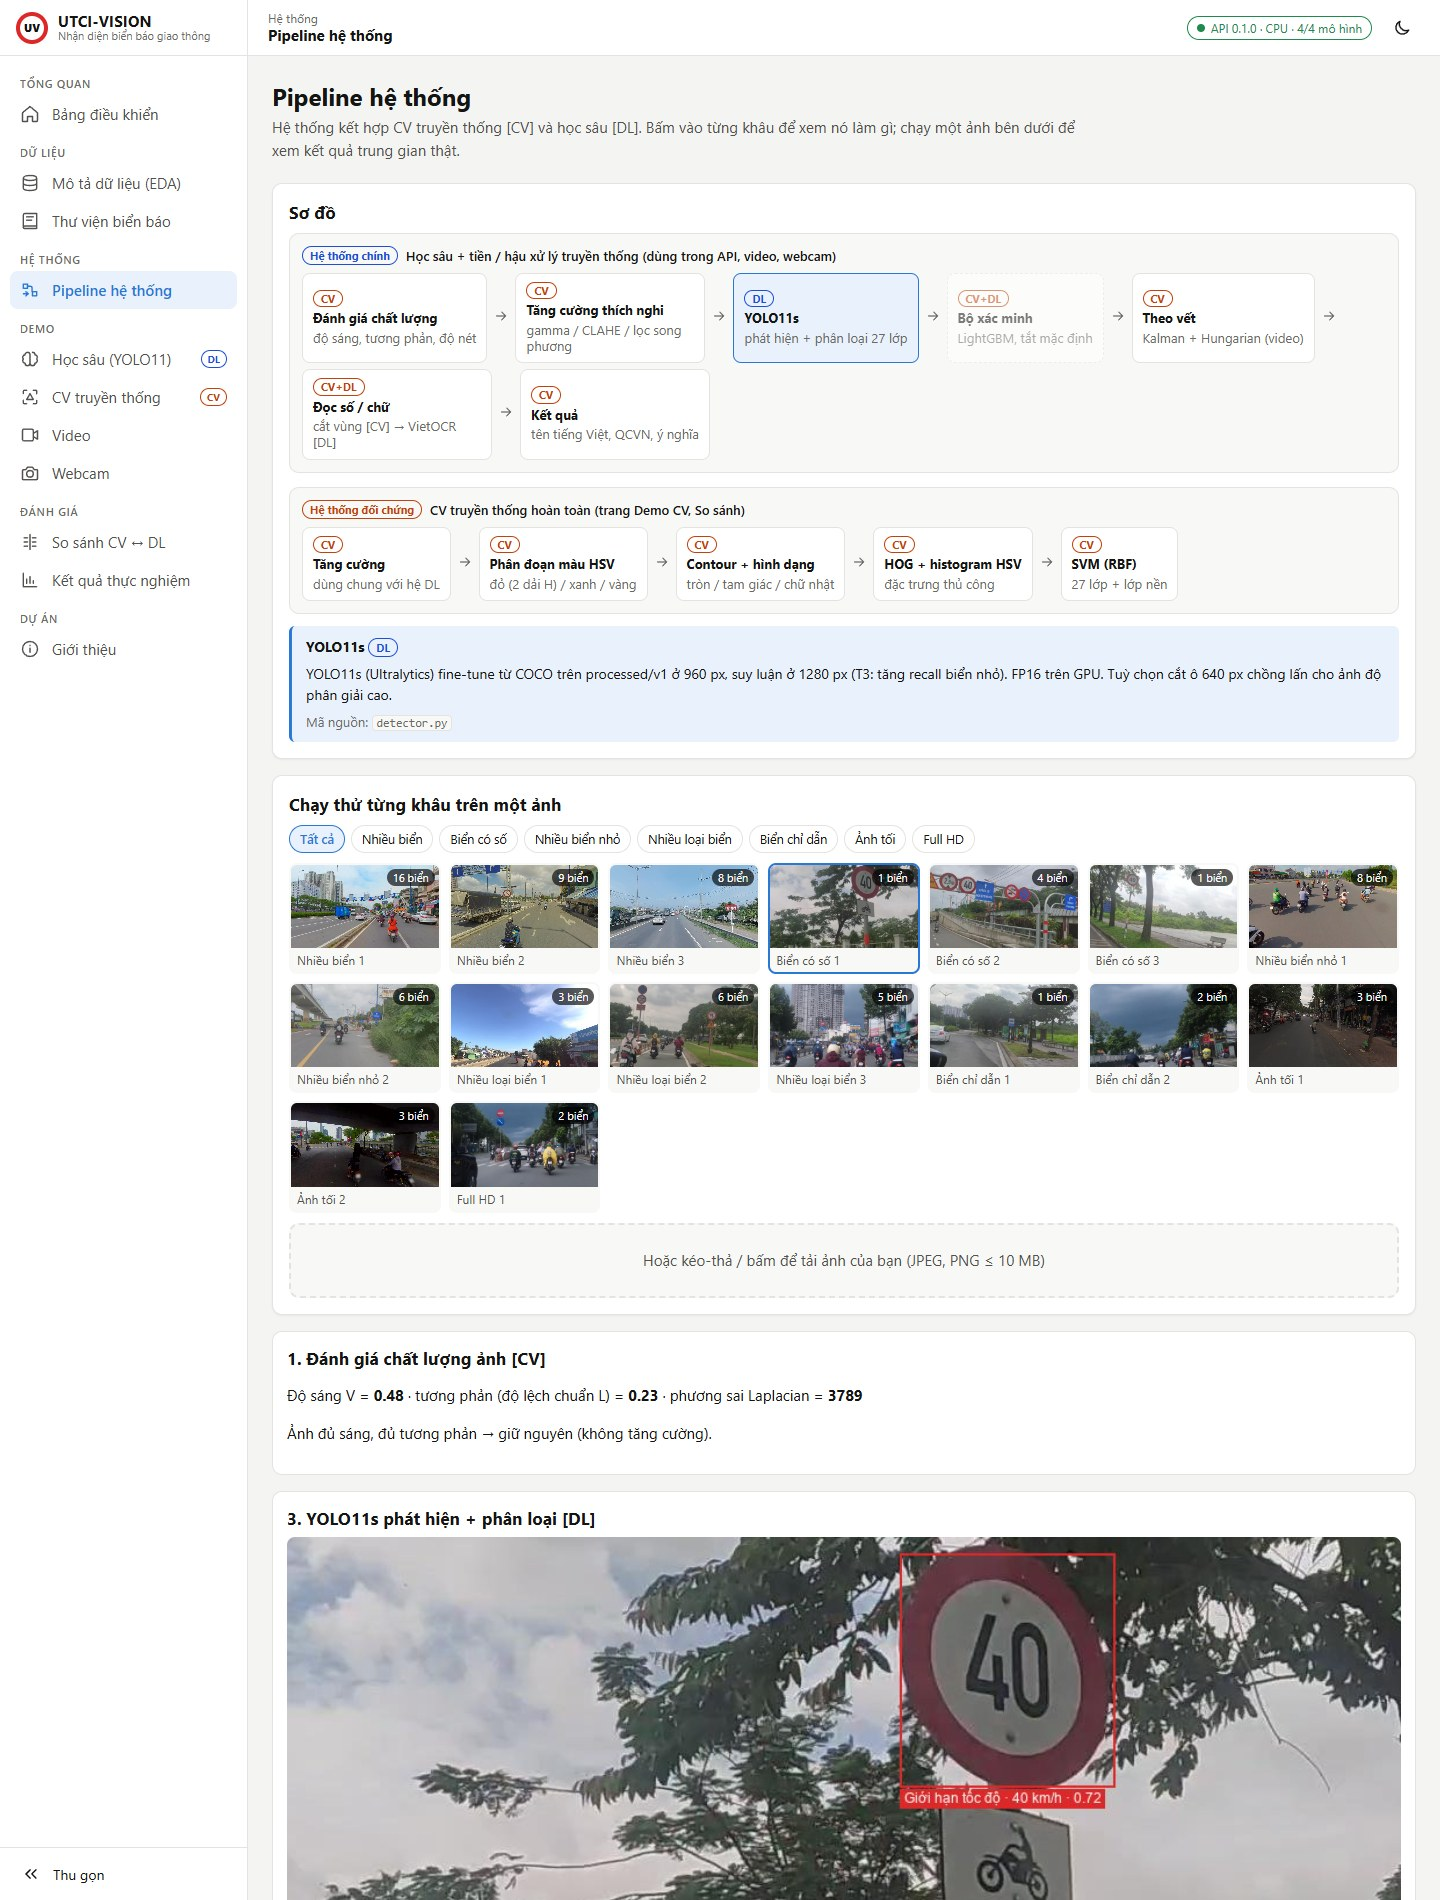
\includegraphics[width=.86\textwidth]{figures/web_pipeline.jpg}
\caption{Trang Pipeline hệ thống: sơ đồ tương tác và kết quả trung gian của từng khâu}
\label{fig:web_pipeline}
\end{figure}

Hình~\ref{fig:web_dl} là trang Demo học sâu với ảnh có nhiều biển nhỏ: người dùng chọn kích thước suy luận, bật/tắt từng khâu và mô phỏng điều kiện xấu; kết quả hiển thị danh sách biển theo nhóm, mã QCVN và thời gian của từng khâu. Đây là cách trình diễn trực tiếp các thí nghiệm T3, T4 và E2.

\begin{figure}[H]
\centering
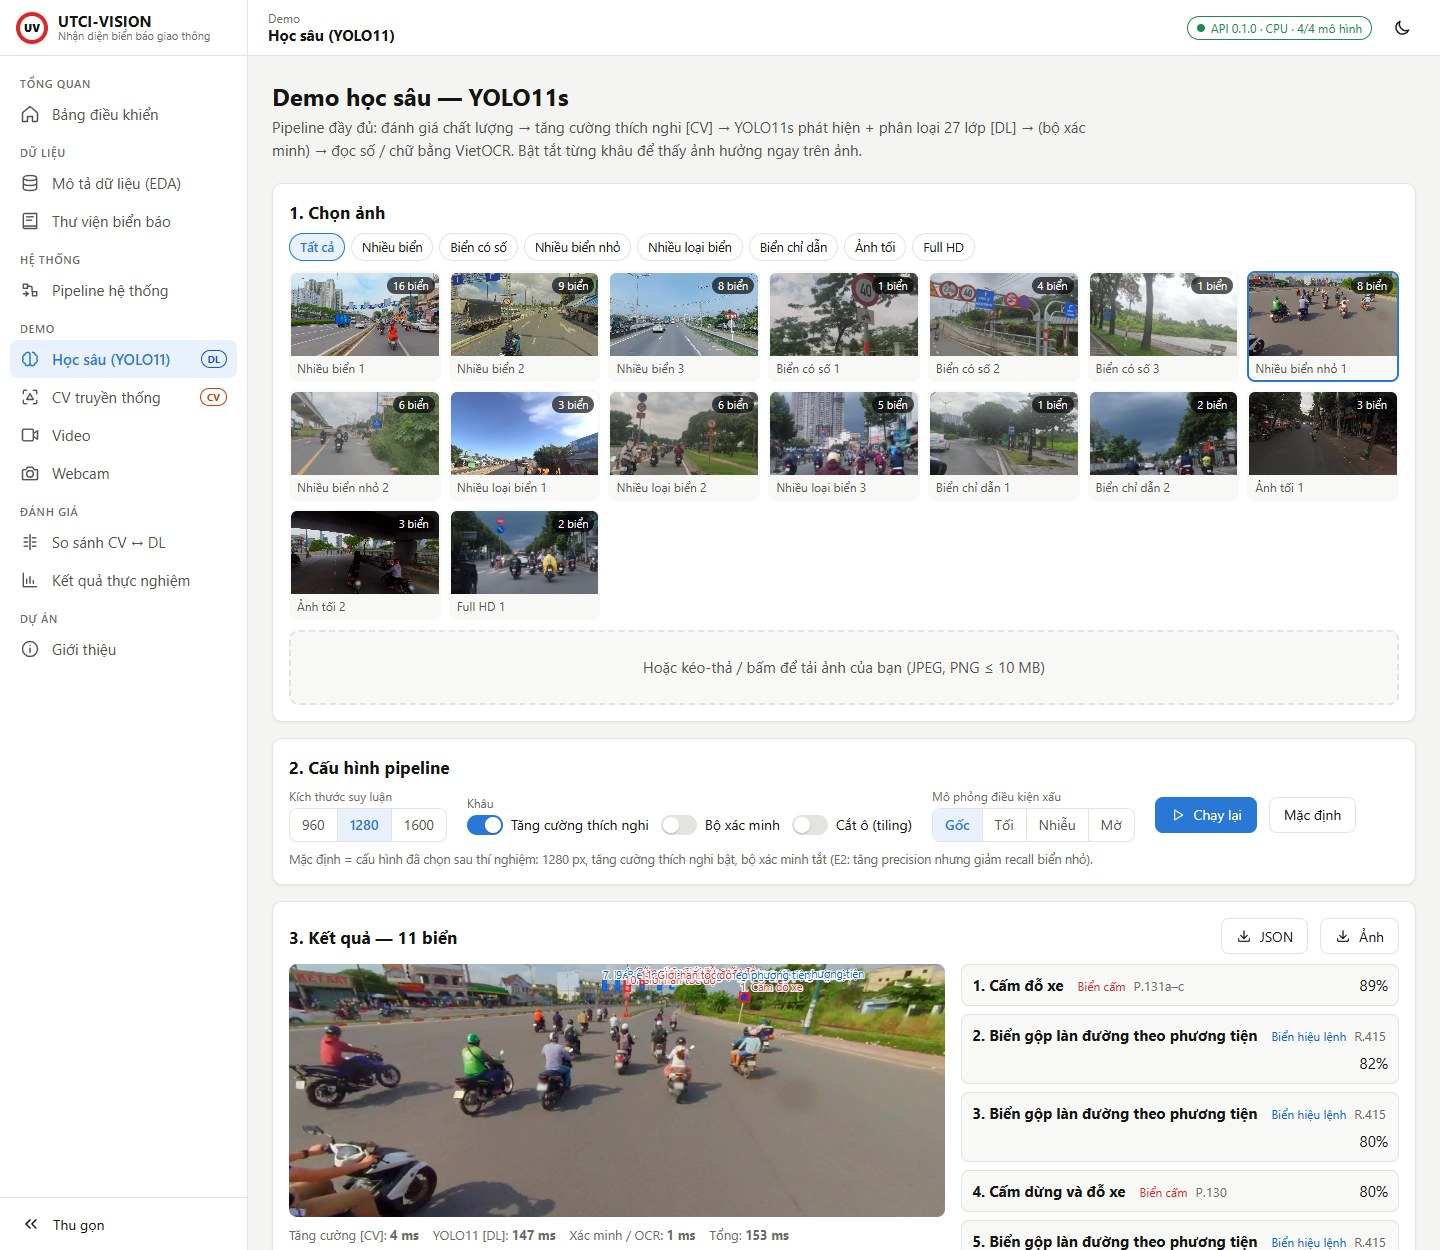
\includegraphics[width=.86\textwidth]{figures/web_dl.jpg}
\caption{Trang Demo học sâu: cấu hình pipeline và kết quả trên ảnh có nhiều biển nhỏ}
\label{fig:web_dl}
\end{figure}

Hình~\ref{fig:web_cv} là trang Demo CV truyền thống, hiển thị lần lượt ảnh đầu vào, mặt nạ màu HSV, vùng ứng viên và kết quả; thời gian từng bước và chỉ số chất lượng ảnh được ghi ngay dưới ảnh. Hình~\ref{fig:web_compare} là trang So sánh, chạy cả hai hệ thống trên cùng ảnh và lập bảng so khớp trên từng biển mà YOLO tìm thấy.

\begin{figure}[H]
\centering
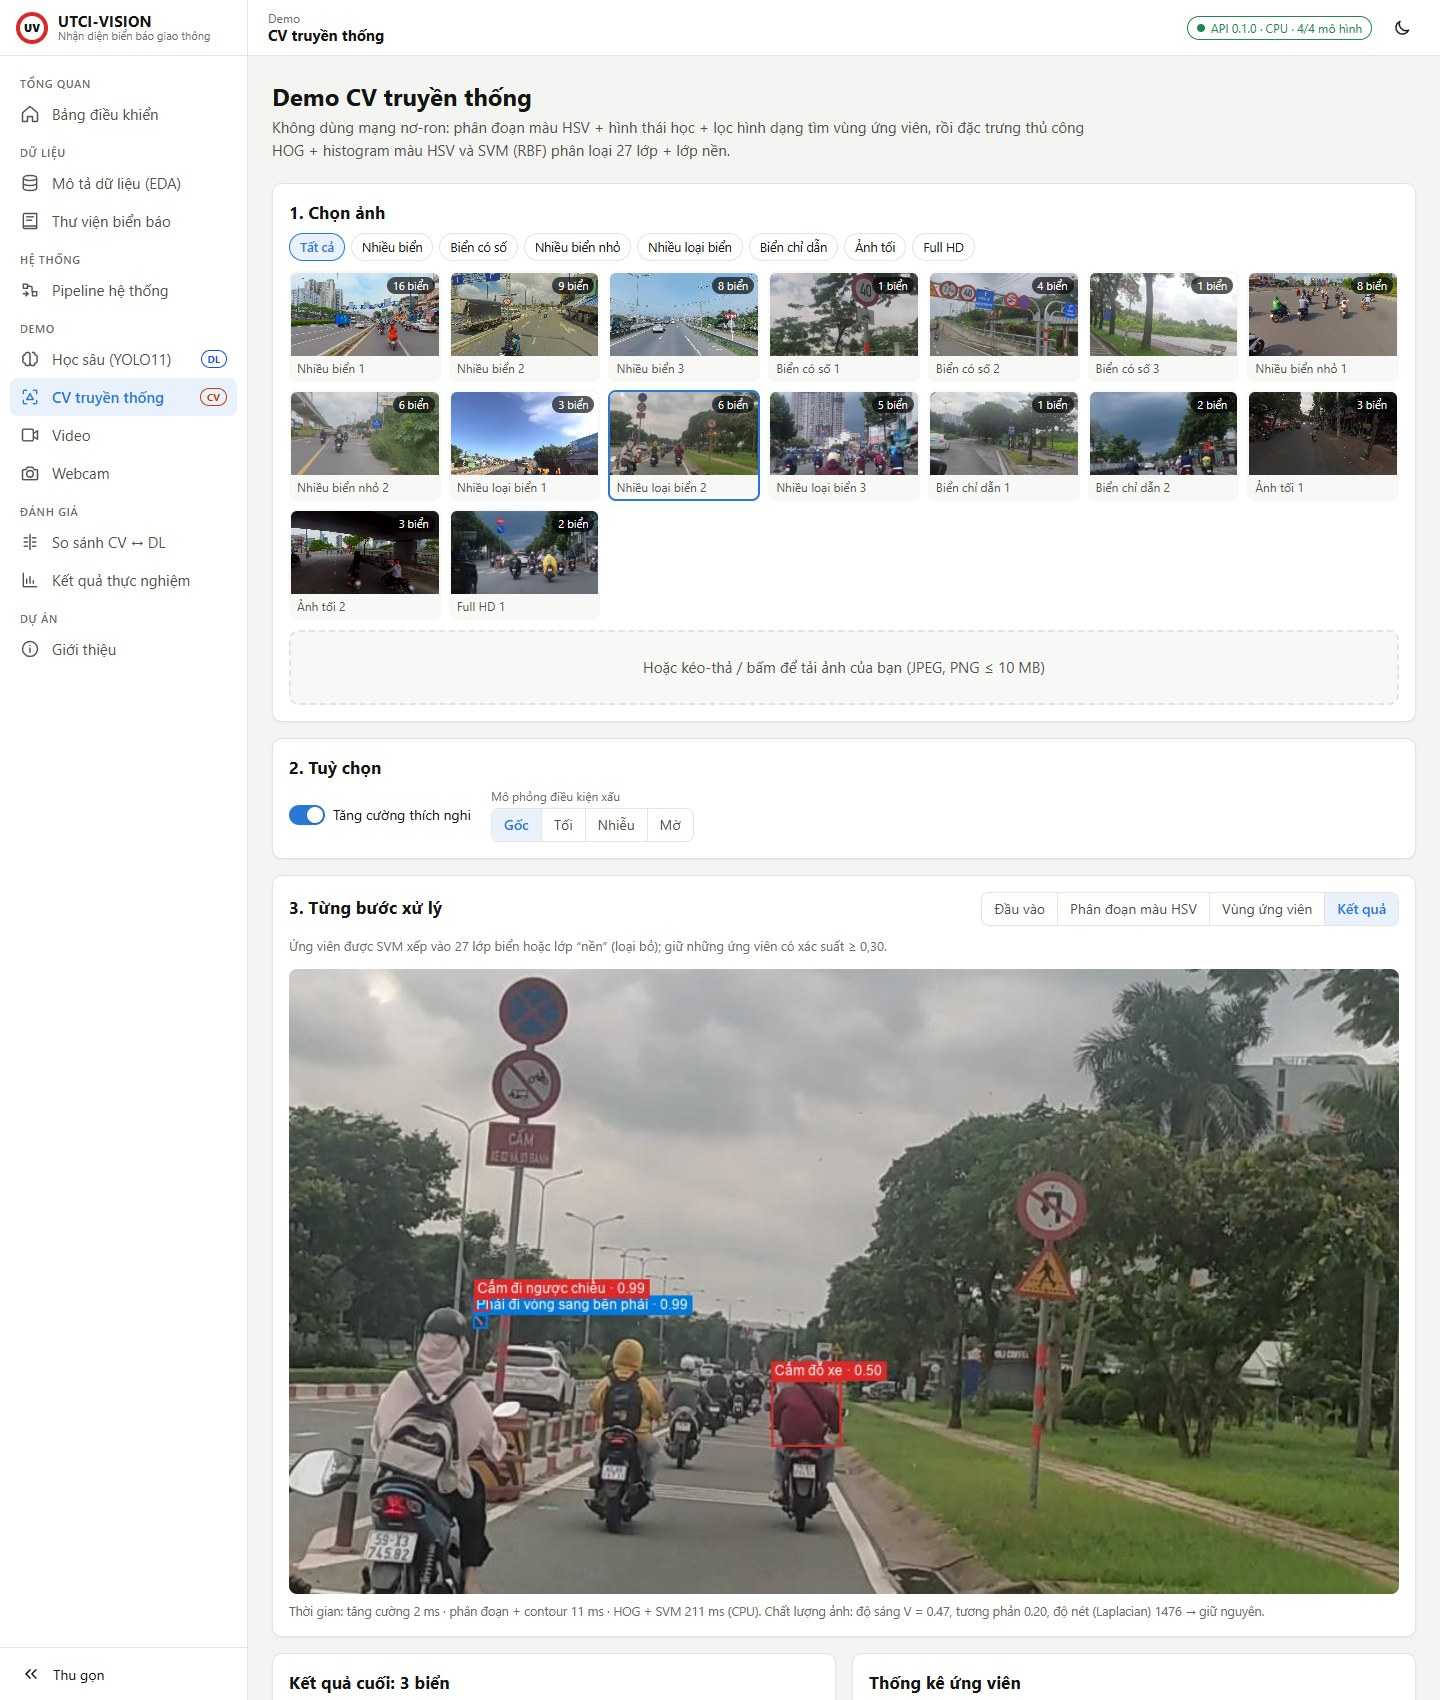
\includegraphics[width=.86\textwidth]{figures/web_cv.jpg}
\caption{Trang Demo CV truyền thống: kết quả của pipeline màu + hình dạng + HOG + SVM}
\label{fig:web_cv}
\end{figure}

\begin{figure}[H]
\centering
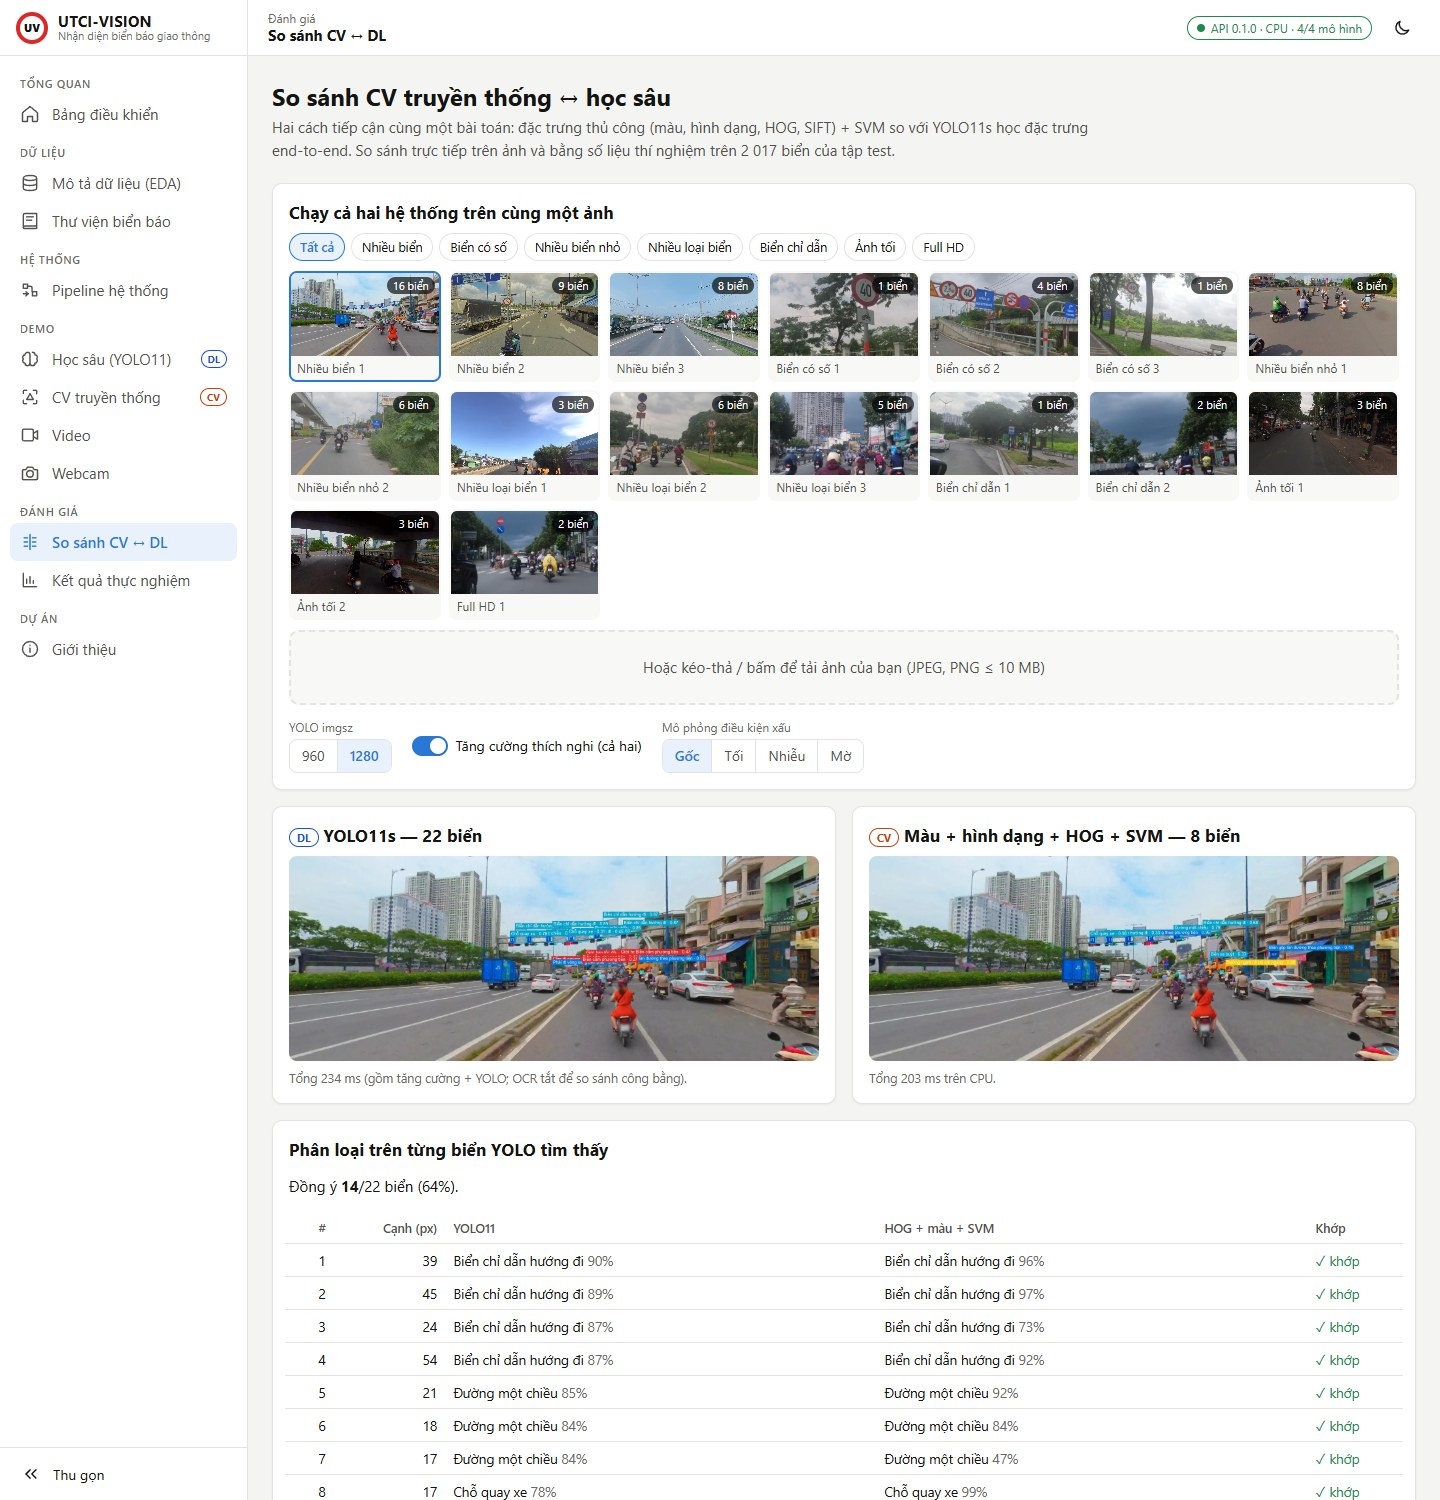
\includegraphics[width=.86\textwidth]{figures/web_compare.jpg}
\caption{Trang So sánh CV -- DL: hai hệ thống trên cùng ảnh và bảng so khớp từng biển}
\label{fig:web_compare}
\end{figure}

\section{Thảo luận}
\label{sec:discussion}

\subsection{Trả lời các câu hỏi đặt ra}
\begin{itemize}
 \item \textbf{Học sâu hay đặc trưng thủ công?} Ở khâu phân loại, HOG + màu + SVM chỉ kém YOLO11s 1,4 điểm và ngang YOLO trên biển nhỏ đã được định vị. Khoảng cách lớn nằm ở khâu định vị: phân đoạn màu và lọc hình dạng sinh nhiều báo động giả và bỏ sót biển. Vì vậy, YOLO11s là lõi của hệ thống, còn đặc trưng thủ công là phương pháp đối chứng có giá trị giải thích.
 \item \textbf{Xử lý ảnh truyền thống đóng góp gì trong hệ thống học sâu?} Tăng cường thích nghi là đóng góp đo được rõ nhất (recall ảnh rất tối 0,686 $\rightarrow$ 0,822), với điều kiện có bước đánh giá chất lượng đứng trước. Bộ xác minh bằng đặc trưng thủ công không cải thiện thật. Theo vết và cắt vùng chữ là các khâu cần thiết về chức năng nhưng chưa đo định lượng được.
 \item \textbf{Cải thiện biển nhỏ khi không thể thêm dữ liệu?} Suy luận ở độ phân giải cao hơn độ phân giải huấn luyện là cách rẻ và hiệu quả nhất (+10,3 điểm recall biển nhỏ, không mất precision); cắt ô tăng recall thêm nhưng đổi lại precision và tốc độ.
\end{itemize}

\subsection{Về việc đánh giá}
Kết quả cho thấy cần thận trọng với con số tổng. Precision của thư viện (0,920) khác precision tại ngưỡng thật (0,860); mAP trên dữ liệu cùng nguồn (khoảng 0,89--0,91) khác kết quả trên cảnh ít tương đồng (precision 0,749); một khâu tăng precision có thể chỉ là dịch điểm vận hành. Đánh giá theo kích thước, theo lớp, theo mức tương đồng và so sánh ở cùng recall với khoảng tin cậy giúp tránh các kết luận sai này. Các con số của công trình khác (ví dụ YOLOv5 trên biển Việt Nam~\cite{tung2024vietnam,cu2024vietnamese}) dùng dữ liệu, cách chia và chỉ số khác nên không so sánh trực tiếp với kết quả của đề tài.

\subsection{Hạn chế}
\label{sec:limitations}
\begin{itemize}
 \item \textbf{Một lần huấn luyện, một trọng số.} Chưa có nhiều hạt giống để ước lượng biến động do huấn luyện; tập xác thực đã dùng để chọn epoch YOLO và học bộ xác minh.
 \item \textbf{Dữ liệu cùng nguồn, đã đóng băng.} Không có tập kiểm thử ngoài phân phối; nhãn có lỗi hệ thống đã biết (lớp ``Biển chỉ dẫn hướng đi''); không có nhãn chữ nên không đo được độ chính xác đọc số và chữ.
 \item \textbf{Ảnh xấu là giả lập.} Ảnh làm tối khác ảnh đêm thật (đèn xe, đèn đường, nhiễu cảm biến); ngưỡng tối $\mu_V<0{,}30$ còn bỏ sót ảnh tối và nên được chọn lại trên tập xác thực.
 \item \textbf{Video và webcam.} Độ ổn định nhãn khi có theo vết chưa đo được vì chưa có video đường phố thật; webcam thời gian thực cần GPU và chưa thử với camera thật.
 \item \textbf{Phiên bản quy chuẩn.} Danh mục lớp và ý nghĩa biển theo QCVN~41:2019/BGTVT; quy chuẩn này đã được thay bằng QCVN~41:2024/BGTVT từ ngày 01/01/2025~\cite{qcvn41_2019}, nên phần ý nghĩa và mã hiệu cần được rà soát lại.
\end{itemize}
